\section{User Study}
	\label{sec:user_study}
	\subsection{Overview}
	A study was performed in which the change in user engagement was evaluated upon being presented with interactive and non-interactive advertisements. In order to accurately estimate user engagement, we measured two primary known indicators: the participants' time perception \citep{time_perception}, and attention \cite{what_is_engagement}. Time perception was recorded directly via participants' verbal responses, while attention was assessed via information recall -- shown by \citet{interactions_attention_memory} to strongly correlate with attention, and used previously also by \citet{advertising_engagement} to measure engagement.

	\subsection{Methodology}
	Out of a set of 119 student targeted adverts provided from Project4, 8 were given interactive html/css overlays containing responsive content likely to be typical for an interactive TV advert. To minimise the problem of a user needing to interact with an overlay for longer than length of the advert, they were designed using techniques discussed by \citet{integrated-approach-advertising}. The interactive content added is given in Table~\ref{tab:interactive_content}.

	\begin{table}[hb]
		\centering
		\begin{tabularx}{\linewidth}{ >{\centering}X X }
			\toprule
			\bf Product & \bf Interactive content \\
			\midrule
			Pot Noodles & \textbf{Poll}: The user may vote for their favourite flavour of Pot Noodle, and is thanked upon doing so. \\
			Smirnoff Vodka & \textbf{Social}: The user may `Like' Smirnoff Vodka, as if via the social networking website Facebook. \\
			`The Perks of Being a Wallflower' (movie) & \textbf{Information}: The user may enter their postcode, causing a map to display the locations of nearby cinema showings. \\
			Scotland Holidays & \textbf{Information}: The user may enter their email address to request more holiday-related information. \\
			Foster's Lager & \textbf{Social}: The user may `Like' Foster's Lager, as if via the social networking website Facebook. \\
			Unified Insurance Cover & \textbf{Information}: The user may select \newline possessions they own, and are given an estimated insurance quote. \\
			Domino's Pizza & \textbf{Purchase}: The user may interact with the advert as if to order a pizza. \\
			\url{thetrainline.com} & \textbf{Poll}: The user may vote on if they think train tickets are too expensive, and are shown poll results upon voting. \\
			\bottomrule
		\end{tabularx}
		\caption{Interactive content added to advertisements}
		\label{tab:interactive_content}
	\end{table}

	Each participant in the study was shown two rounds of adverts---one interactive and one non-interactive---with half the participants being shown the interactive adverts first, and the other half shown non-interactive adverts first. The length of the rounds varied between 4, 5, and 6 minutes, and were evenly split between longer interactive rounds, longer non-interactive rounds and equal length rounds; the purpose of which was to measure differences in the participants perceived time and actual round time. 

	The study followed a pre-prepared script, as included in Appendix~\ref{sec:appendix_interview_script}. While participants were neither encouraged nor discouraged from interacting with the overlays on the set of modified adverts, they were informed that interactions were possible in order to help ameliorate the effects of any initial learning period. As part of the study, video introductions were given for each section, as scripted in Appendix~\ref{sec:appendix_video_script}.

	\subsection{Results}

	%Introduction - we carried out the survey, and got some results
	%Justification - these results were interesting, highlights
	%Conclusion - Results are good, mmkay?

	% Time perception
	For question 2b, participants were asked ``\textit{Please estimate how much time more or less you were watching in the second session?}''. Figure~\ref{fig:time_perception} displays the recorded responses, showing the amount that users over/underestimated the time spent watching each round of advertisements, and an extrapolated normal distribution.

	\begin{figure}[!h]
		\centering
		\begin{subfigure}[h]{0.49\textwidth}
			\centering
			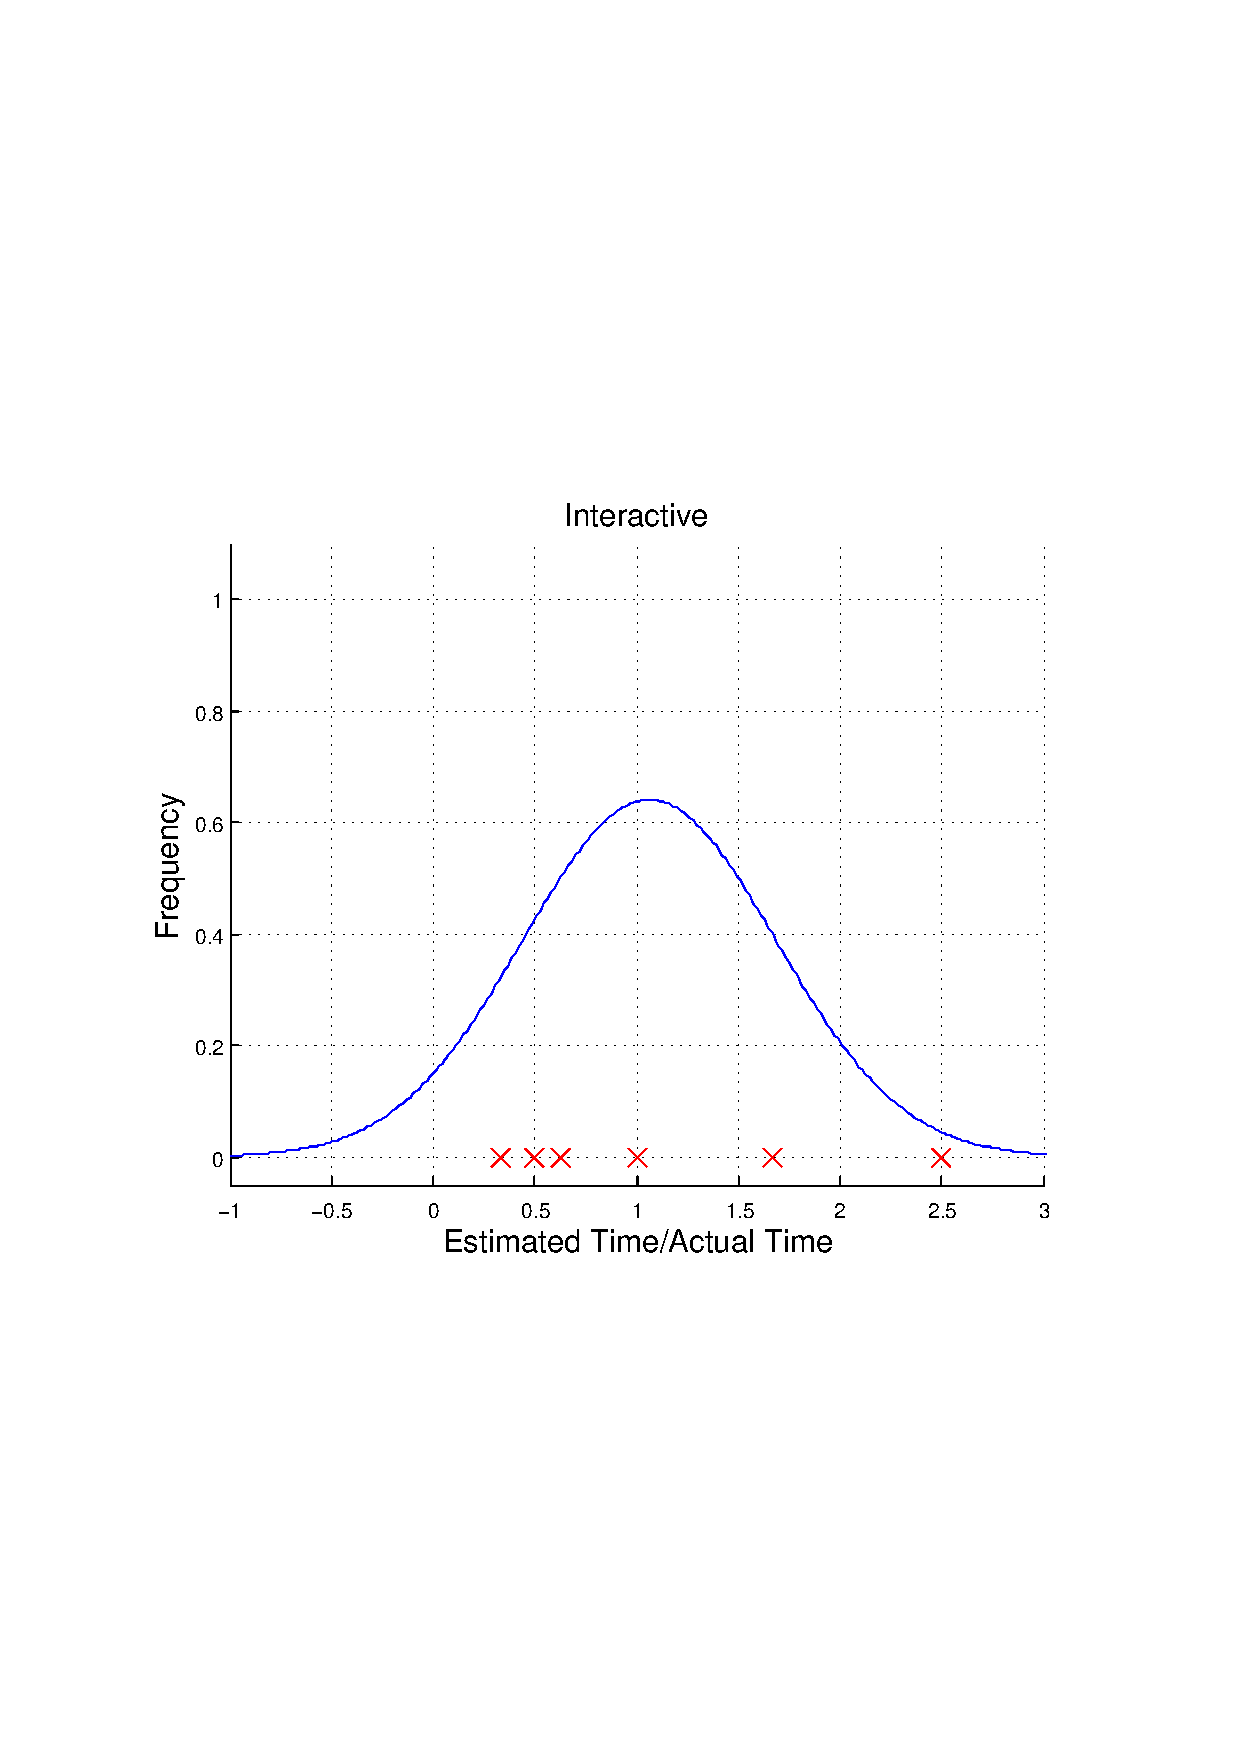
\includegraphics[width=\textwidth]{images/interactive_bell.pdf}
			\caption{Interactive adverts: $\mu$~=~1.0625, $\sigma$~=~0.6228}
		\end{subfigure}
		\begin{subfigure}[h]{0.49\textwidth}
			\centering
			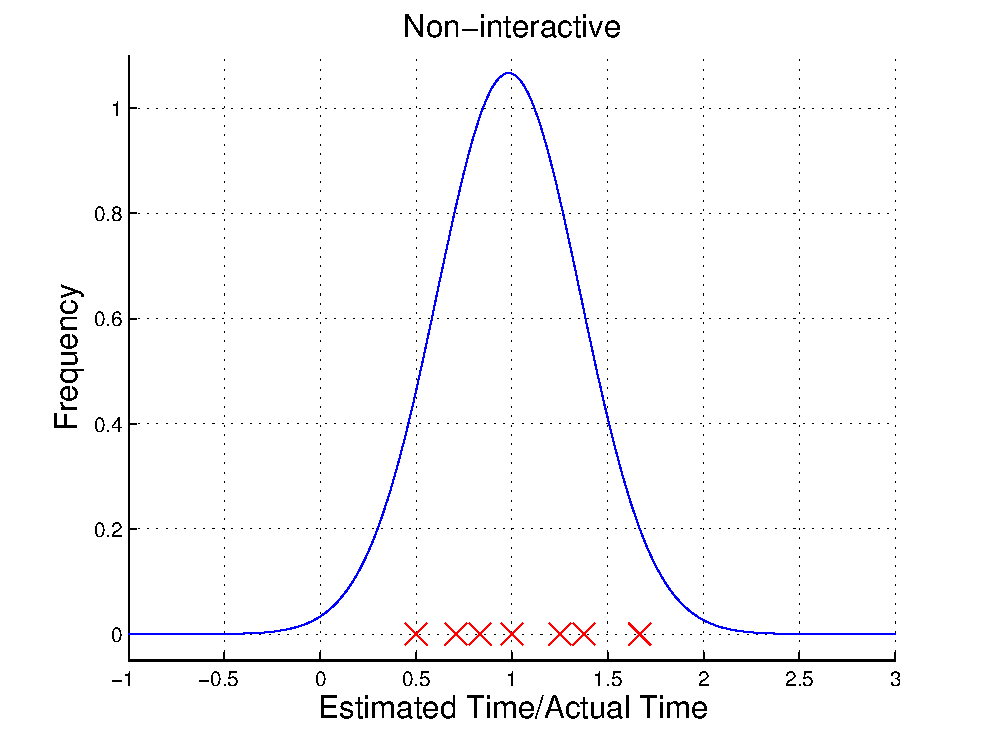
\includegraphics[width=\textwidth]{images/noninteractive_bell.pdf}
			\caption{Non-interactive adverts: $\mu=0.9833$, $\sigma=0.3739$}
		\end{subfigure}
		\caption{Errors in time estimations of users watching interactive and non-interactive advertisements, and extrapolated normal distributions. 10 points recorded in study used.}
		\label{fig:time_perception}
	\end{figure}
	Little difference in time perception between interactive and non-interactive advertisements is shown by Figure~\ref{fig:time_perception}. A Student's independent two-sample t-test performed on the time estimate data gives 0.17, showing strong support for the null hypothesis that there is no significant difference in the time perception error between interactive and non-interactive advertisements.

	% Recall
	Using information in the participants' answers, a table was constructed of adverts that were recalled by participants and whether the participants had seen the advert in the interactive round, the non-interactive round or both rounds. The recall results are given in Figure~\ref{fig:recall}, where it can be seen that participants had a better recall of adverts from the noninteractive round. 

	\begin{figure}[!h]
		\centering
		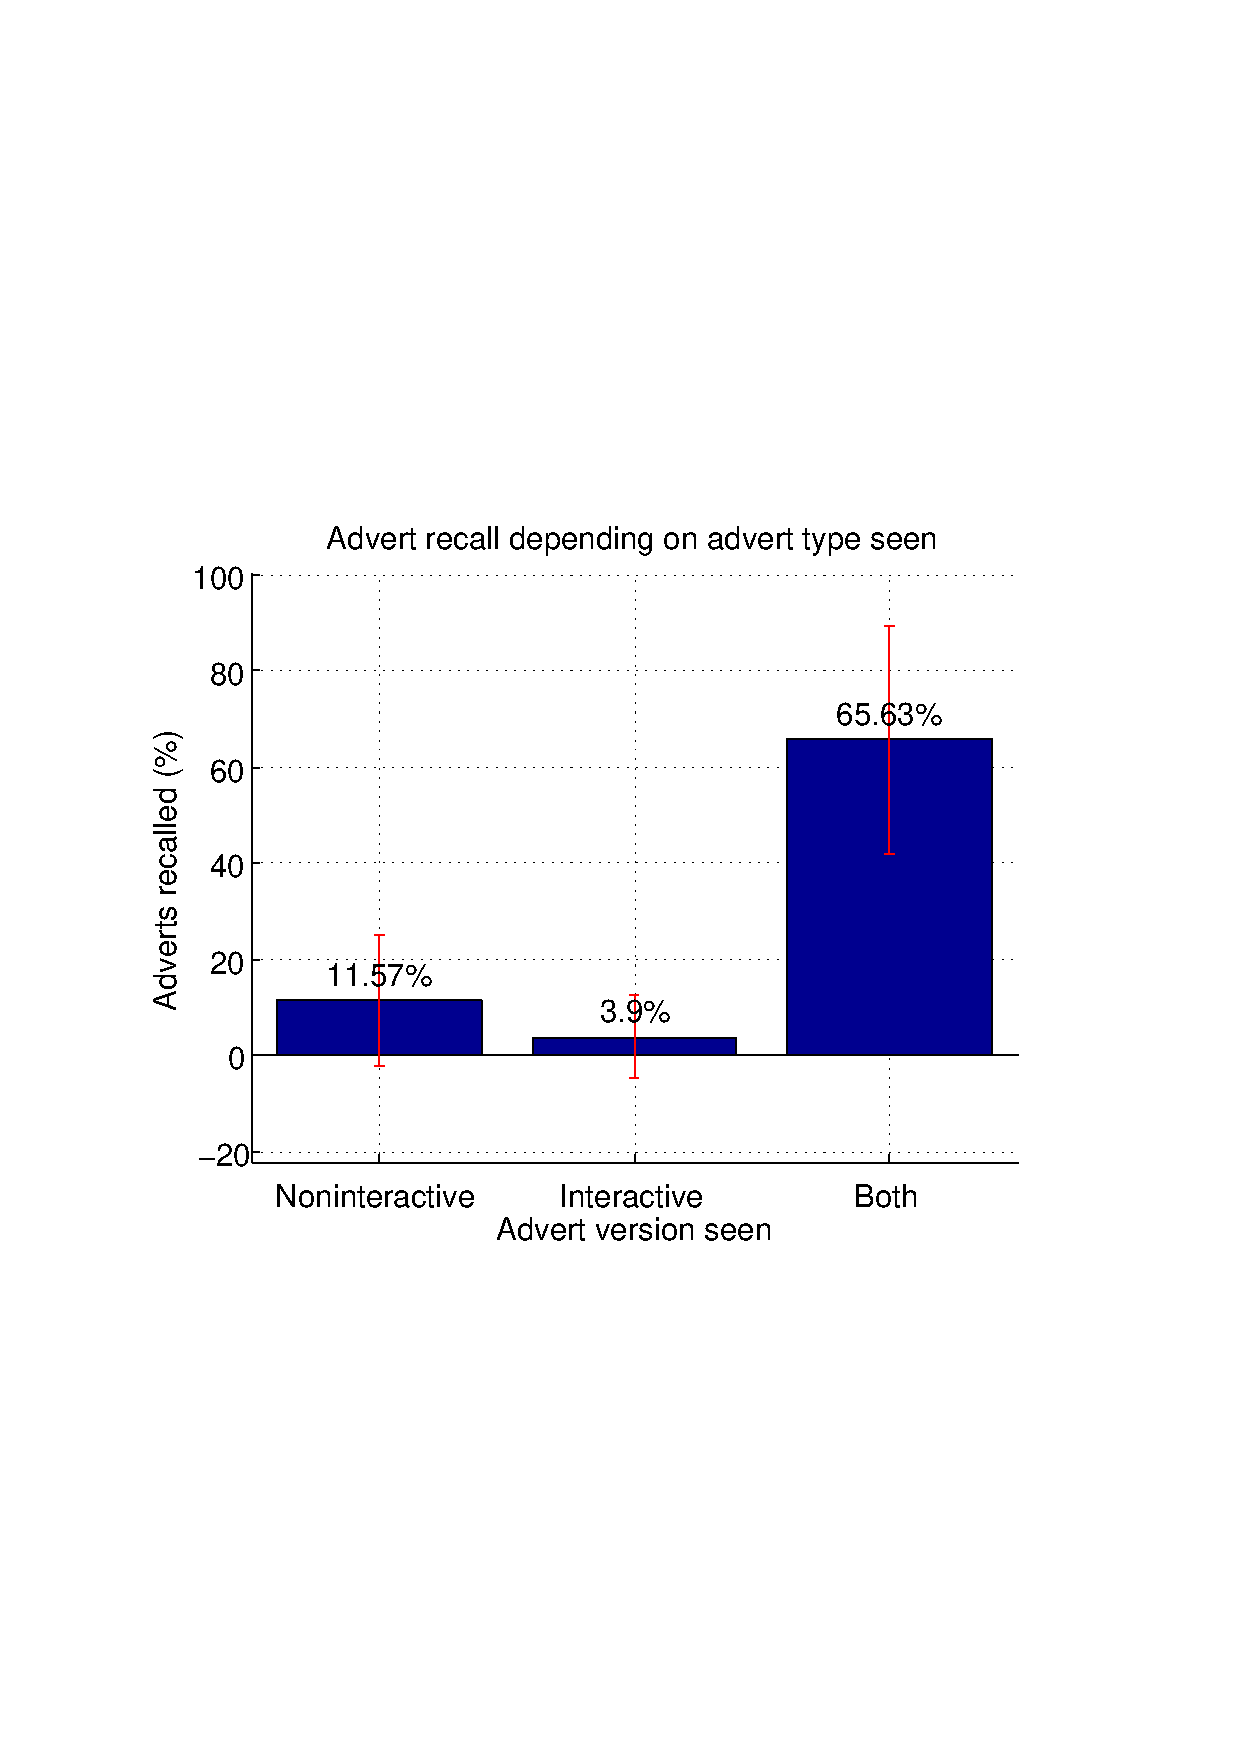
\includegraphics[width=\textwidth]{images/recall.pdf}
		\caption{Average percentage of advertisements recalled depending on the version of the advert seen (interactive, non-interactive or both versions). The red error bars indicate the mean recall rate $\pm$ one standard deviation.}
		\label{fig:recall}
	\end{figure}

	Along with taking quantitative measurements of time perception and information recall, data was also collected on how participants believed they perceived the interactive and noninteractive adverts differently. This data was collected during the interview stage from participant answers. Questions 3, 4, 5, 6, and 9 were polar (yes/no questions), and the percentage of positive results have been given in Figure~\ref{fig:yesno_results}. The significant results that can be seen from Figure~\ref{fig:yesno_results} are: participants believe that advert relevance leads to heightened attention and likelihood of being watched, and that interactivity in adverts leads to heightened enjoyment. Results which are less significant and with greater variance are: interactive adverts are paid slightly more attention, and are enjoyed marginally less than non-interactive versions.

	\begin{figure}[h!]
		\centering
		\begin{subfigure}[t]{0.49\textwidth}
			\centering
			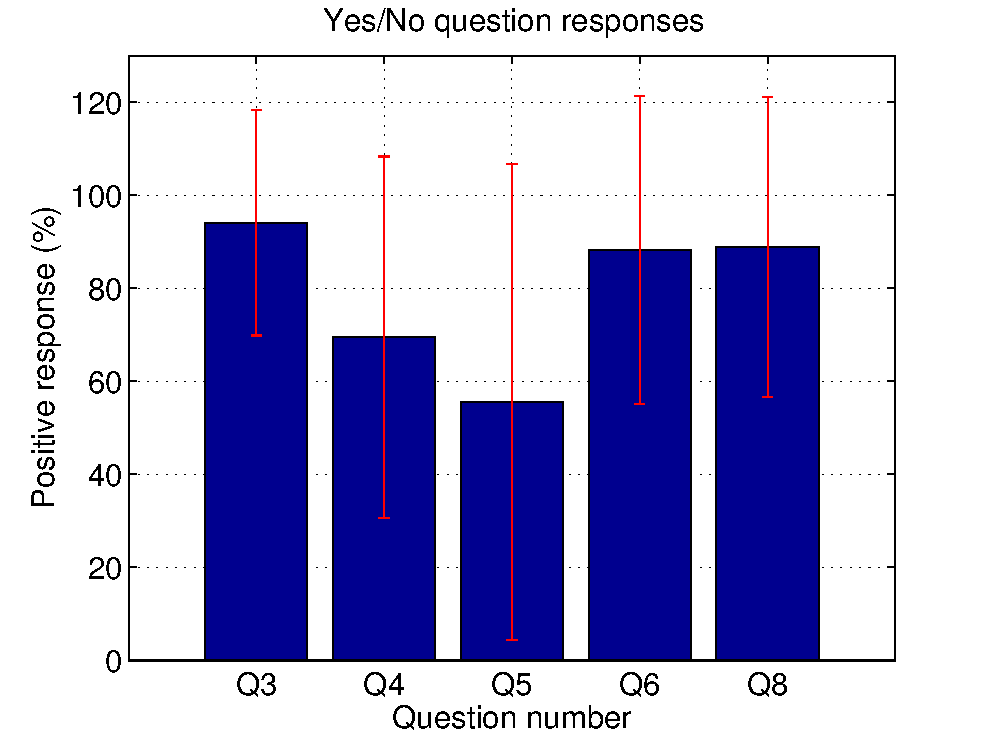
\includegraphics[width=\textwidth]{images/yesno_results.pdf}
			\caption{Positive responses to yes/no questions. \\
				(Q3) More attention paid to relevant ads. \\
				(Q4) More attention paid to interactive ads. \\
				(Q5) Remember more of interactive ads. \\
				(Q6) Enjoyed interactive ads more. \\
				(Q9) More likely to watch relevant ads.
			}
			\label{fig:yesno_results}
		\end{subfigure}
		\begin{subfigure}[t]{0.49\textwidth}
			\centering
			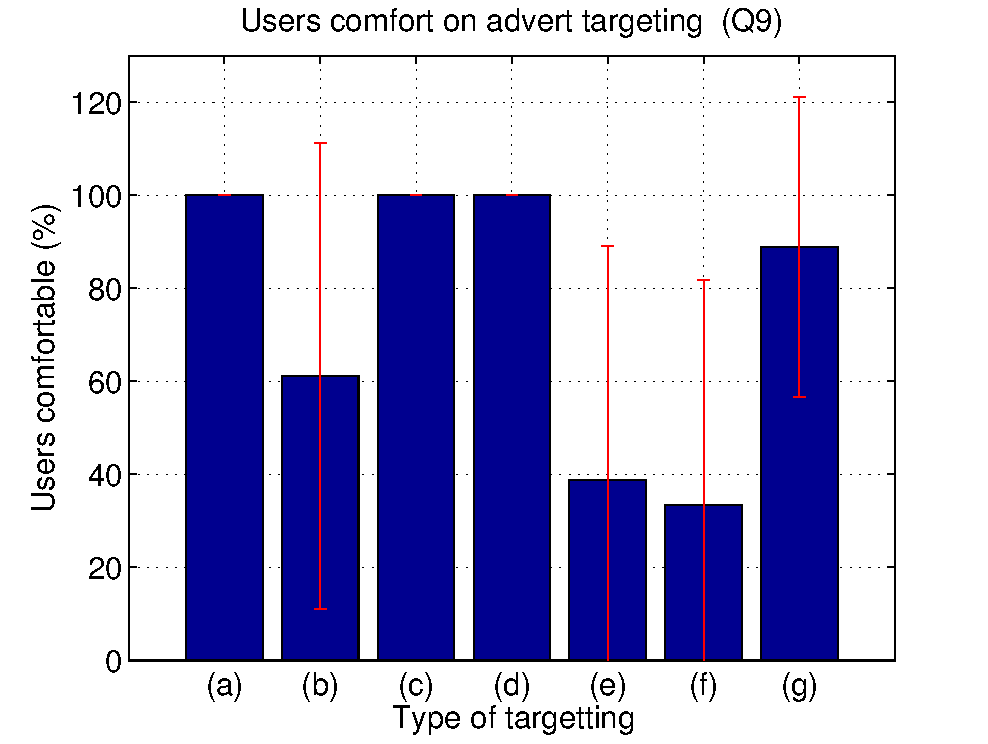
\includegraphics[width=\textwidth]{images/targeting.pdf}
			\caption{(Q10) Percentages of users who reported to be comfortable with different advert targeting information sources. (a) Anonymous \\demographics. (b) Current location. \\(c) Current time. (d) Playlist content. \\(e) Internet browsing history. (f) Facebook information. (g) User preference information learned by the system.}
		\end{subfigure}
		\caption{Analysis of positive user responses to a number of polar questions. The red error bars indicate the mean values $\pm$ one standard deviation.}
		\label{fig:qualitative_results}
	\end{figure}


	%71\% of participants showed an improvement in engagement, 

	%where engagements is the average of attention (q4), memororability (q5) and enjoyment (q6)

	%i.e., avg(69.4, 55.6, 88.2) = 71.1\%

	%I made this equation up, but would be good if we could back this up. Perhaps with \citep{what_is_engagement}
